\chapter{Implementation of the Agents}
\label{implOfAgents}
In this project, the RL agents are designed such that their functionality is encapsulated within a top-level scene called \texttt{Main.tscn}. Within this scene, there is an instance of the selected agent, and the code makes use of several functions implemented by the agent in order to interact with the environment. Specifically, the required functions are: \texttt{move()}, \texttt{init()}, \texttt{start\_game()}, \texttt{end\_game()}, \texttt{save()}, \texttt{set\_seed\_val()}, \texttt{get\_and\_set\_agent\_specific\_parameters()}, and \texttt{get\_n()}.

The purpose of most of these functions is self-explanatory. \texttt{init()} and \texttt{save()} are used to initialize and save the agent's internal state, respectively, and are called only once per experiment. \texttt{start\_game()} and \texttt{end\_game()} are called at the beginning and end of each episode, while \texttt{move()} is called by the \texttt{Tunnels.gd} script, and it is in this function that the agent makes a decision about which action to take based on the current state and score. The remaining functions pertain to the internal structure of the agent and are not relevant to the reader.

\section{Hierarchy}
\begin{figure}[h]
    \centering
    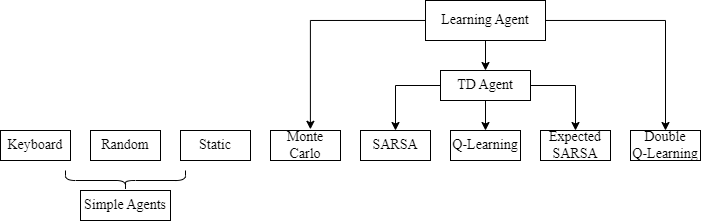
\includegraphics[width=0.8\textwidth]{agents_tree}
    \caption{Agents hierarchy inside the project}
    \label{fig:agents_tree}
\end{figure}

In the current design of the game, there are a total of 8 agents implemented, 5 of which utilize some form of reinforcement learning (RL) algorithm. These RL agents share a common superclass called ``Learning Agent'', while 3 of them are further subclassed under the ``TD Agent'' class (see Figure \ref{fig:agents_tree}). As previously discussed, the RL algorithms can be broadly divided into two categories: Monte Carlo methods and temporal difference (TD) learning. The TD algorithms differ only in their update function, and so it was deemed appropriate to group them under the same superclass. However, the Double Q-Learning agent, which utilizes separate policies and requires additional modifications, was implemented as a separate subclass or the ``Learning Agent''. The implementation details of these agents will be further elaborated upon in the subsequent sections. 

Before proceeding further, it is crucial to emphasize that, as previously mentioned when describing the state in Chapter 3, the agent has the ability to perform movements in various directions, including moving right, forward, or left, and each of these movements can be performed in combination with shooting. Therefore, on each time step, the move function of the agent returns a list of two elements: the first element signifies the movement direction, where a value of -1 represents left, 0 represents forward, and 1 represents right; while the second element determines whether the agent will shoot or not, with a value of 1 indicating yes and 0 indicating no for shooting.


\section{Simple Agents}
To facilitate testing of the game environment, several simple agents were implemented. These agents serve as baseline models and are used to ensure that the environment is functioning as intended before more sophisticated RL agents are developed. There are three simple agents in total: a ``Keyboard agent'' that receives input from the player via the keyboard, a ``Static agent'' that always chooses the forward action without shooting, and a ``Random agent'' that chooses a random action at each time step. 

\section{Learning Agent}
The Learning Agent class serves as a base class for all the reinforcement learning agents in this project. It provides a set of shared functions and features that are used by all agents, such as reading and writing data to a file and debugging statements. In terms of decision-making, these agents all follow an $\epsilon$-greedy policy, whereby they select the action with the highest value for a given state with a certain probability, or randomly choose any action with the remaining probability. Each of the subclasses of the Learning Agent class then implements specific code that is unique to that particular agent.

\begin{algorithm}
\caption{Choosing an action using $\epsilon$-greedy policy}
\begin{algorithmic}[1]
\Function{choose\_action}{action}
    \State $\textit{epsilon\_action} \gets \textit{false}$
    \If{not $\textit{is\_eval\_game}$} \Comment{Used for continuous evaluation}
        \State $\textit{epsilon\_action} \gets rand.\text{randf\_range}(0,1) < EPSILON$
        \If{$\textit{epsilon\_action}$}
            \State $action \gets ACTIONS [rand.\text{randi\_range}(0,len(ACTIONS) - 1)]$  
        \EndIf
    \EndIf
    \State \Return $action$
\EndFunction
\end{algorithmic}
\end{algorithm}

\subsection{Common parameters and behaviours}
In regards to the present implementation of the reinforcement learning algorithms for the 3D tunnel game, certain aspects of the game learning step and parameter implementation are unique to this project and merit discussion. For instance, we should look into the learning step in the game. The agent will not request a new move until the state has changed, despite the fact that it may seem more natural for a new decision to be made on every game tick. This has the effect of reducing the number of decisions that the agent must make in a given episode, but also results in intriguing policy behaviours that are elaborated upon in Chapter \ref{experiments_chapter}.

Furthermore, there are several parameters that are common to all learning agents, some of which were briefly discussed in the preceding chapter. In this section, we will examine in more detail how these parameters were integrated into this particular project. The initial optimistic value parameter is the simplest one to explain, as it is implemented in a straightforward manner. In particular, each time a state-action pair is added to the policy, its value is set to a predetermined number. This number (\texttt{initOptVal}), along with other parameters mentioned subsequently in this subsection, are part of the sub-options agent's parameter that is specified through the command line (see \ref{commOpt}).

The following two parameters worth noting are \texttt{eps} and \texttt{epsFinal}, which are responsible for the random moves executed by the $\epsilon$-greedy policy. These parameters allow the user to specify the starting and ending values of $\epsilon$, which are then suitably decreased after each game played. The formula for this decrease is as follows: $$decrease = (\frac{epsFinal}{eps})^{\frac{1.0}{n}}$$

Here, \texttt{n} represents the number of games being played. The reason behind this epsilon decrease is to change the ratio between exploration and exploitation over time. At the beginning of the experiment, the \texttt{eps} value is higher, and thus random moves happen more often, causing the agent to try actions it would otherwise oversee. Later, when the policy is a bit stabilized, the \texttt{eps} value becomes smaller so it would allow the agent to play longer games and possibly win (if the \texttt{eps} value was high throughout the whole experiment, the agent would have a bigger chance of choosing an inadequate move and thus untimely ending the game).

Finally, it is pertinent to discuss the discounting value gamma (defined by \texttt{gam}). In this project, discounting is used in the following manner: $$\gamma^{next\_step.time - curr\_step.time}$$

Normally, the gamma value grows by one power on each step. However, as previously stated, learning steps in this implementation do not occur on every tick, but instead occur when the state changes. As a result, they may vary in size. To avoid uneven discounting, the time is calculated for each new decision made by the agent using the formula provided:  $$(game.num\_of\_ticks * 33) / 1000.0$$

\subsection{Monte Carlo Agent}

\begin{algorithm}
\caption{Updating policy for Monte Carlo}\label{mcUpdate}
\begin{algorithmic}[1]
\State $R \gets \text{next\_step.score - curr\_step.score}$
\State $G \gets $\Call {pow}{GAMMA,next\_step.time - curr\_step.time} $\cdot (R + G)$
\If{\Call{is\_first\_occurrence}{\dots}}
\State $total\_return[curr\_step.\text{state\_action}] \gets total\_return[curr\_step.\text{state\_action}] + G$
\State $visits[curr\_step.\text{state\_action}] \gets visits[curr\_step.\text{state\_action}] + 1$
\EndIf
\end{algorithmic}
\end{algorithm}

The Monte Carlo method is a type of reinforcement learning algorithm that updates its policy only after an episode is completed. This is done by iterating through the entire episode and increasing the number of visits and total return for each state-action pair, if this is their first visit inside this episode. The total return is calculated using the formula shown in the Algorithm \ref{mcUpdate}, while the number of visits is simply incremented by 1. To determine the optimal action, the agent compares the ratio of total return to number of visits for each possible action at a given state. This calculation is performed at each state transition during the episode \footnote{Instead of calling the move function periodically, the agents will always choose the same action based on the current state. Only once the state has changed, the new action is chosen based on the accumulated score and the new state.}.
As previously mentioned, the $\gamma$ variable in the equation shown in \ref{mcUpdate} serves as a discount factor, meaning that the last move made, which resulted in the agent's death, will receive the highest penalty. As we move further down the list of moves, their significance decreases. It is important to note that if the value of $\gamma$ is set to 1, all moves are given equal weight. 

\subsection{TD Agent}	
Unlike the Monte Carlo methods, which update their policies only after the completion of an episode, TD agents update their policies in real-time, after each action is taken. To accomplish this, all TD agents have a shared function called \texttt{move()}, which call the function displayed in \ref{tdUpdate}. 

\begin{algorithm}
\caption{Updating policy for TD Agent}\label{tdUpdate}
\begin{algorithmic}[1]
\State $ alpha \gets 1.0 / visits[last\_state\_action]$
\State $new\_state\_val \gets new\_state\_action$
\If {terminal}:
\State $new\_state\_val \gets0$
\EndIf
\State $new\_gamma \gets $\Call {pow}{GAMMA,curr\_time - prev\_time}
\State $q[last\_state\_action] \gets q[last\_state\_action] + alpha(new\_gamma(R + new\_state\_val) - q[last\_state\_action])$
\end{algorithmic}
\end{algorithm}


The update of the policy for a specific state value in TD learning involves multiple variables, most of which have been previously discussed. One new variable is $\alpha$, which represents the total number of visits for a given state action pair divided by one. Furthermore, to make this calculation, a variable uniquely computed by each TD algorithm, known as \texttt{new\_state\_action}, is required. Various methods for computing this variable can be found in Algorithms \ref{sUpdate}, \ref{qUpdate} and \ref{esUpdate}. If the current state is a terminal state, the \texttt{new\_state\_action} will not be utilized and instead, it will be replaced with a value of 0, as indicated in the update code.

\begin{algorithm}
\caption{Update function for SARSA}\label{sUpdate}
\begin{algorithmic}[1]
\Function{get\_update}{$state, new\_action, \_best\_action$}
\State \textbf{return} $q[\text{get\_state\_action}(state, new\_action)]$
\EndFunction
\end{algorithmic}
\end{algorithm}

\begin{algorithm}
\caption{Update function for Q-Learning}\label{qUpdate}
\begin{algorithmic}[1]
\Function{get\_update}{$state, \_new\_action, best\_action$}
\State \textbf{return} $q[\Call{get\_state\_action}{state, best\_action}]$
\EndFunction
\end{algorithmic}
\end{algorithm}

\begin{algorithm}
\caption{Update function for ExpectedSARSA}\label{esUpdate}
\begin{algorithmic}[1]
\Function{get\_update}{$state, \_new\_action, best\_action$}
\State $sum \gets 0.0$
\For{$action$ \textbf{in} $ACTIONS$}
\State $probability \gets \frac{EPSILON}{\text{len}(ACTIONS)}$
\If{$action = best\_action$}
\State $probability \gets probability + 1 - EPSILON$
\EndIf
\State $sum \gets sum + probability \cdot Q(state, action)$
\EndFor
\State \Return $sum$
\EndFunction
\end{algorithmic}
\end{algorithm}

In SARSA, the \texttt{new\_state\_val} is calculated based on the value of the next action the agent will take, denoted as \texttt{new\_action}. On the other hand, Q-learning uses the value of the best action possible in the next state, denoted as \texttt{best\_action}. These two variables are equal if greedy policy is implemented. However if we consider $\epsilon$-greedy policy, then they might differ based on weather a random action has been chosen. Expected SARSA combines these two approaches by taking the expected value of all possible actions in the next state. 

\begin{algorithm}
\caption{Update function for Double Q-Learning}\label{dqlUpdate}
\begin{algorithmic}
\State $ alpha \gets 1.0 / visits[last\_state\_action]$
\State $ new\_gamma \gets $\Call {pow}{GAMMA,next\_step.time - curr\_step.time}
\If{$rand.\text{randf\_range}(0,1) < 0.5$}
\State $new\_state\_val \gets q2[\text{get\_state\_action}(state,best\_action)]$
\If {terminal}:
\State $new\_state\_val \gets0$
\EndIf
\State $ q[last\_state\_action] \gets alpha(new\_gamma(R + new\_state\_val) - q[last\_state\_action])$
\Else
\State $new\_state\_val \gets q[\text{get\_state\_action}(state,best\_action)]$
\If {terminal}:
\State $new\_state\_val \gets0$
\EndIf
\State $ q2[last\_state\_action] \gets alpha(new\_gamma(R + new\_state\_val) - q2[last\_state\_action])$
\EndIf
\end{algorithmic}
\end{algorithm}

Similar to the agents in the TD class, the update for the Double Q-Learning agent occurs each time the agent changes its state. The update process is slightly different. In this method, two separate action-value functions, denoted as Q1 and Q2, are used to estimate the maximum action value for a given state. At each update step, one of the Q-values is selected randomly and updated using the other Q-value as a reference. This process helps to reduce the overestimation of action values and leads to more stable learning.